%%%%%%%%%%%%%%%%%%%%%%%%%%%%%%%%%%%%%%%%%
% Style based on: The Legrand Orange Book - Version 1.4 (12/4/14)
%
% The original template has been downloaded from:
% http://www.LaTeXTemplates.com
%
% Original author:
% Mathias Legrand (legrand.mathias@gmail.com)
%
% License:
% CC BY-NC-SA 3.0 (http://creativecommons.org/licenses/by-nc-sa/3.0/)
%%%%%%%%%%%%%%%%%%%%%%%%%%%%%%%%%%%%%%%%%

%----------------------------------------------------------------------------------------
%	PACKAGES AND OTHER DOCUMENT CONFIGURATIONS
%----------------------------------------------------------------------------------------

\documentclass[11pt,fleqn,oneside,openany]{book} % Default font size and left-justified equations

\usepackage[top=3cm,bottom=3cm,left=3.2cm,right=3.2cm,headsep=10pt,a4paper]{geometry} % Page margins

\usepackage{xcolor} % Required for specifying colors by name
\definecolor{ocre}{RGB}{243,102,25} % Define the orange color used for highlighting throughout the book
\definecolor{brown}{RGB}{192,81,20} % Define the brown color used for highlighting of URLs throughout the book

% Font Settings
\usepackage{avant} % Use the Avantgarde font for headings
%\usepackage{times} % Use the Times font for headings
\usepackage{mathptmx} % Use the Adobe Times Roman as the default text font together with math symbols from the Sym­bol, Chancery and Com­puter Modern fonts

\usepackage{microtype} % Slightly tweak font spacing for aesthetics
\usepackage[utf8]{inputenc} % Required for including letters with accents
\usepackage[T1]{fontenc} % Use 8-bit encoding that has 256 glyphs

% For fancy verbatim environment with code highlights.
\usepackage{fancyvrb}
\usepackage{color}
\newcommand\codeHighlightRed[1]{\textcolor[rgb]{1,0,0}{\textbf{#1}}}
\newcommand\codeHighlightDarkRed[1]{\textcolor[rgb]{0.65,0,0}{\textbf{#1}}}
\newcommand\codeHighlightBrown[1]{\textcolor[rgb]{0.9,0.68,0.49}{\textbf{#1}}}
\newcommand\codeHighlightGreen[1]{\textcolor[rgb]{0.4,0.6,0.3}{\textbf{#1}}}
\newcommand\codeHighlightBlue[1]{\textcolor[rgb]{0,0,1}{\textbf{#1}}}
\newcommand\codeHighlightPurple[1]{\textcolor[rgb]{0.68,0,1}{\textbf{#1}}}

% Bibliography
%\usepackage[style=alphabetic,sorting=nyt,sortcites=true,autopunct=true,babel=hyphen,hyperref=true,abbreviate=false,backref=true,backend=biber]{biblatex}
%\addbibresource{bibliography.bib} % BibTeX bibliography file
%\defbibheading{bibempty}{}

% Index
%\usepackage{calc} % For simpler calculation - used for spacing the index letter headings correctly
%\usepackage{makeidx} % Required to make an index
%\makeindex % Tells LaTeX to create the files required for indexing

%----------------------------------------------------------------------------------------
%	VARIOUS REQUIRED PACKAGES
%----------------------------------------------------------------------------------------

\usepackage{titlesec} % Allows customization of titles

\usepackage{graphicx} % Required for including images
\graphicspath{{images/}} % Specifies the directory where images are stored

\usepackage{lipsum} % Inserts dummy text

\usepackage{tikz} % Required for drawing custom shapes

\usepackage[english]{babel} % English language/hyphenation

\usepackage{enumitem} % Customize lists
\setlist{nolistsep} % Reduce spacing between bullet points and numbered lists

\usepackage{booktabs} % Required for nicer horizontal rules in tables

\usepackage{eso-pic} % Required for specifying an image background in the title page

%----------------------------------------------------------------------------------------
%	MAIN TABLE OF CONTENTS
%----------------------------------------------------------------------------------------

\usepackage{titletoc} % Required for manipulating the table of contents

\contentsmargin{0cm} % Removes the default margin
% Chapter text styling
\titlecontents{chapter}[1.25cm] % Indentation
{\addvspace{15pt}\large\sffamily\bfseries} % Spacing and font options for chapters
{\color{ocre!60}\contentslabel[\Large\thecontentslabel]{1.25cm}\color{ocre}} % Chapter number
{}  
{\color{ocre!60}\normalsize\sffamily\bfseries\;\titlerule*[.5pc]{.}\;\thecontentspage} % Page number
% Section text styling
\titlecontents{section}[1.25cm] % Indentation
{\addvspace{5pt}\sffamily\bfseries} % Spacing and font options for sections
{\contentslabel[\thecontentslabel]{1.25cm}} % Section number
{}
{\sffamily\hfill\color{black}\thecontentspage} % Page number
[]
% Subsection text styling
\titlecontents{subsection}[1.25cm] % Indentation
{\addvspace{1pt}\sffamily\small} % Spacing and font options for subsections
{\contentslabel[\thecontentslabel]{1.25cm}} % Subsection number
{}
{\sffamily\;\titlerule*[.5pc]{.}\;\thecontentspage} % Page number
[] 

%----------------------------------------------------------------------------------------
%	MINI TABLE OF CONTENTS IN CHAPTER HEADS
%----------------------------------------------------------------------------------------

% Section text styling
\titlecontents{lsection}[0em] % Indendating
{\footnotesize\sffamily} % Font settings
{}
{}
{}

% Subsection text styling
\titlecontents{lsubsection}[.5em] % Indentation
{\normalfont\footnotesize\sffamily} % Font settings
{}
{}
{}
 
%----------------------------------------------------------------------------------------
%	PAGE HEADERS
%----------------------------------------------------------------------------------------

\usepackage{fancyhdr} % Required for header and footer configuration

\pagestyle{fancy}
\renewcommand{\chaptermark}[1]{\markboth{\sffamily\normalsize\bfseries\chaptername\ \thechapter.\ #1}{}} % Chapter text font settings
\renewcommand{\sectionmark}[1]{\markright{\sffamily\normalsize\thesection\hspace{5pt}#1}{}} % Section text font settings
\fancyhf{} \fancyhead[LE,RO]{\sffamily\normalsize\thepage} % Font setting for the page number in the header
\fancyhead[LO]{\rightmark} % Print the nearest section name on the left side of odd pages
\fancyhead[RE]{\leftmark} % Print the current chapter name on the right side of even pages
\renewcommand{\headrulewidth}{0.5pt} % Width of the rule under the header
\addtolength{\headheight}{2.5pt} % Increase the spacing around the header slightly
\renewcommand{\footrulewidth}{0pt} % Removes the rule in the footer
\fancypagestyle{plain}{\fancyhead{}\renewcommand{\headrulewidth}{0pt}} % Style for when a plain pagestyle is specified

% Removes the header from odd empty pages at the end of chapters
\makeatletter
\renewcommand{\cleardoublepage}{
\clearpage\ifodd\c@page\else
\hbox{}
\vspace*{\fill}
\thispagestyle{empty}
\newpage
\fi}

%----------------------------------------------------------------------------------------
%	THEOREM STYLES
%----------------------------------------------------------------------------------------

\usepackage{amsmath,amsfonts,amssymb,amsthm} % For math equations, theorems, symbols, etc

\newcommand{\intoo}[2]{\mathopen{]}#1\,;#2\mathclose{[}}
\newcommand{\ud}{\mathop{\mathrm{{}d}}\mathopen{}}
\newcommand{\intff}[2]{\mathopen{[}#1\,;#2\mathclose{]}}
\newtheorem{notation}{Notation}[chapter]

%%%%%%%%%%%%%%%%%%%%%%%%%%%%%%%%%%%%%%%%%%%%%%%%%%%%%%%%%%%%%%%%%%%%%%%%%%%
%%%%%%%%%%%%%%%%%%%% dedicated to boxed/framed environements %%%%%%%%%%%%%%
%%%%%%%%%%%%%%%%%%%%%%%%%%%%%%%%%%%%%%%%%%%%%%%%%%%%%%%%%%%%%%%%%%%%%%%%%%%
\newtheoremstyle{ocrenumbox}% % Theorem style name
{0pt}% Space above
{0pt}% Space below
{\normalfont}% % Body font
{}% Indent amount
{\small\bf\sffamily\color{ocre}}% % Theorem head font
{\;}% Punctuation after theorem head
{0.25em}% Space after theorem head
{\small\sffamily\color{ocre}\thmname{#1}\nobreakspace\thmnumber{\@ifnotempty{#1}{}\@upn{#2}}% Theorem text (e.g. Theorem 2.1)
\thmnote{\nobreakspace\the\thm@notefont\sffamily\bfseries\color{black}---\nobreakspace#3.}} % Optional theorem note
\renewcommand{\qedsymbol}{$\blacksquare$}% Optional qed square

\newtheoremstyle{blacknumex}% Theorem style name
{5pt}% Space above
{5pt}% Space below
{\normalfont}% Body font
{} % Indent amount
{\small\bf\sffamily}% Theorem head font
{\;}% Punctuation after theorem head
{0.25em}% Space after theorem head
{\small\sffamily{\tiny\ensuremath{\blacksquare}}\nobreakspace\thmname{#1}\nobreakspace\thmnumber{\@ifnotempty{#1}{}\@upn{#2}}% Theorem text (e.g. Theorem 2.1)
\thmnote{\nobreakspace\the\thm@notefont\sffamily\bfseries---\nobreakspace#3.}}% Optional theorem note

\newtheoremstyle{blacknumbox} % Theorem style name
{0pt}% Space above
{0pt}% Space below
{\normalfont}% Body font
{}% Indent amount
{\small\bf\sffamily}% Theorem head font
{\;}% Punctuation after theorem head
{0.25em}% Space after theorem head
{\small\sffamily\thmname{#1}\nobreakspace\thmnumber{\@ifnotempty{#1}{}\@upn{#2}}% Theorem text (e.g. Theorem 2.1)
\thmnote{\nobreakspace\the\thm@notefont\sffamily\bfseries---\nobreakspace#3.}}% Optional theorem note

%%%%%%%%%%%%%%%%%%%%%%%%%%%%%%%%%%%%%%%%%%%%%%%%%%%%%%%%%%%%%%%%%%%%%%%%%%%
%%%%%%%%%%%%% dedicated to non-boxed/non-framed environements %%%%%%%%%%%%%
%%%%%%%%%%%%%%%%%%%%%%%%%%%%%%%%%%%%%%%%%%%%%%%%%%%%%%%%%%%%%%%%%%%%%%%%%%%
\newtheoremstyle{ocrenum}% % Theorem style name
{5pt}% Space above
{5pt}% Space below
{\normalfont}% % Body font
{}% Indent amount
{\small\bf\sffamily\color{ocre}}% % Theorem head font
{\;}% Punctuation after theorem head
{0.25em}% Space after theorem head
{\small\sffamily\color{ocre}\thmname{#1}\nobreakspace\thmnumber{\@ifnotempty{#1}{}\@upn{#2}}% Theorem text (e.g. Theorem 2.1)
\thmnote{\nobreakspace\the\thm@notefont\sffamily\bfseries\color{black}---\nobreakspace#3.}} % Optional theorem note
\renewcommand{\qedsymbol}{$\blacksquare$}% Optional qed square
\makeatother

% Defines the theorem text style for each type of theorem to one of the three styles above
\newcounter{dummy} 
\numberwithin{dummy}{section}
\theoremstyle{ocrenumbox}
\newtheorem{theoremeT}[dummy]{Theorem}
\newtheorem{problem}{Problem}[chapter]
\newtheorem{exerciseT}{Exercise}[chapter]
\theoremstyle{blacknumex}
\newtheorem{exampleT}{Example}[chapter]
\theoremstyle{blacknumbox}
\newtheorem{vocabulary}{Vocabulary}[chapter]
\newtheorem{definitionT}{Definition}[section]
\newtheorem{corollaryT}[dummy]{Corollary}
\theoremstyle{ocrenum}
\newtheorem{proposition}[dummy]{Proposition}

%----------------------------------------------------------------------------------------
%	DEFINITION OF COLORED BOXES
%----------------------------------------------------------------------------------------

\RequirePackage[framemethod=default]{mdframed} % Required for creating the theorem, definition, exercise and corollary boxes

% Theorem box
\newmdenv[skipabove=7pt,
skipbelow=7pt,
backgroundcolor=black!5,
linecolor=ocre,
innerleftmargin=5pt,
innerrightmargin=5pt,
innertopmargin=5pt,
leftmargin=0cm,
rightmargin=0cm,
innerbottommargin=5pt]{tBox}

% Exercise box	  
\newmdenv[skipabove=7pt,
skipbelow=7pt,
rightline=false,
leftline=true,
topline=false,
bottomline=false,
backgroundcolor=ocre!10,
linecolor=ocre,
innerleftmargin=5pt,
innerrightmargin=5pt,
innertopmargin=5pt,
innerbottommargin=5pt,
leftmargin=0cm,
rightmargin=0cm,
linewidth=4pt]{eBox}	

% Definition box
\newmdenv[skipabove=7pt,
skipbelow=7pt,
rightline=false,
leftline=true,
topline=false,
bottomline=false,
linecolor=ocre,
innerleftmargin=5pt,
innerrightmargin=5pt,
innertopmargin=0pt,
leftmargin=0cm,
rightmargin=0cm,
linewidth=4pt,
innerbottommargin=0pt]{dBox}	

% Corollary box
\newmdenv[skipabove=7pt,
skipbelow=7pt,
rightline=false,
leftline=true,
topline=false,
bottomline=false,
linecolor=gray,
backgroundcolor=black!5,
innerleftmargin=5pt,
innerrightmargin=5pt,
innertopmargin=5pt,
leftmargin=0cm,
rightmargin=0cm,
linewidth=4pt,
innerbottommargin=5pt]{cBox}

% Creates an environment for each type of theorem and assigns it a theorem text style from the "Theorem Styles" section above and a colored box from above
\newenvironment{theorem}{\begin{tBox}\begin{theoremeT}}{\end{theoremeT}\end{tBox}}
\newenvironment{exercise}{\begin{eBox}\begin{exerciseT}}{\hfill{\color{ocre}\tiny\ensuremath{\blacksquare}}\end{exerciseT}\end{eBox}}
\newenvironment{definition}{\begin{dBox}\begin{definitionT}}{\end{definitionT}\end{dBox}}	
\newenvironment{example}{\begin{exampleT}}{\hfill{\tiny\ensuremath{\blacksquare}}\end{exampleT}}		
\newenvironment{corollary}{\begin{cBox}\begin{corollaryT}}{\end{corollaryT}\end{cBox}}	

%----------------------------------------------------------------------------------------
%	REMARK ENVIRONMENT
%----------------------------------------------------------------------------------------

\newenvironment{remark}{\par\vspace{10pt}\small % Vertical white space above the remark and smaller font size
\begin{list}{}{
\leftmargin=35pt % Indentation on the left
\rightmargin=25pt}\item\ignorespaces % Indentation on the right
\makebox[-2.5pt]{\begin{tikzpicture}[overlay]
\node[draw=ocre!60,line width=1pt,circle,fill=ocre!25,font=\sffamily\bfseries,inner sep=2pt,outer sep=0pt] at (-15pt,0pt){\textcolor{ocre}{R}};\end{tikzpicture}} % Orange R in a circle
\advance\baselineskip -1pt}{\end{list}\vskip5pt} % Tighter line spacing and white space after remark

%----------------------------------------------------------------------------------------
%	SECTION NUMBERING IN THE MARGIN
%----------------------------------------------------------------------------------------

\makeatletter
\renewcommand{\@seccntformat}[1]{\llap{\textcolor{ocre}{\csname the#1\endcsname}\hspace{1em}}}                    
\renewcommand{\section}{\@startsection{section}{1}{\z@}
{-4ex \@plus -1ex \@minus -.4ex}
{1ex \@plus.2ex }
{\normalfont\large\sffamily\bfseries}}
\renewcommand{\subsection}{\@startsection {subsection}{2}{\z@}
{-3ex \@plus -0.1ex \@minus -.4ex}
{0.5ex \@plus.2ex }
{\normalfont\sffamily\bfseries}}
\renewcommand{\subsubsection}{\@startsection {subsubsection}{3}{\z@}
{-2ex \@plus -0.1ex \@minus -.2ex}
{.2ex \@plus.2ex }
{\normalfont\small\sffamily\bfseries}}                        
\renewcommand\paragraph{\@startsection{paragraph}{4}{\z@}
{-2ex \@plus-.2ex \@minus .2ex}
{.1ex}
{\normalfont\small\sffamily\bfseries}}

%----------------------------------------------------------------------------------------
%	HYPERLINKS IN THE DOCUMENTS
%----------------------------------------------------------------------------------------

% For an unclear reason, the package should be loaded now and not later
\usepackage{hyperref}
\hypersetup{hidelinks,backref=true,pagebackref=true,hyperindex=false,
colorlinks=true,breaklinks=true,urlcolor=ocre,linkcolor=black,
bookmarks=true,bookmarksopen=false,pdftitle={Title},pdfauthor={Author}}

%----------------------------------------------------------------------------------------
%	CHAPTER HEADINGS
%----------------------------------------------------------------------------------------

% The set-up below should be (sadly) manually adapted to the overall margin page septup controlled by the geometry package loaded in the main.tex document. It is possible to implement below the dimensions used in the goemetry package (top,bottom,left,right)... TO BE DONE

\newcommand{\thechapterimage}{}
\newcommand{\chapterimage}[1]{\renewcommand{\thechapterimage}{#1}}

% Numbered chapters with mini tableofcontents
\def\thechapter{\arabic{chapter}}
\def\@makechapterhead#1{
\thispagestyle{empty}
{\centering \normalfont\sffamily
\ifnum \c@secnumdepth >\m@ne
\if@mainmatter
\startcontents
\begin{tikzpicture}[remember picture,overlay]
\node at (current page.north west)
{\begin{tikzpicture}[remember picture,overlay]
\node[anchor=north west,inner sep=0pt] at (0,0) {\includegraphics[width=\paperwidth]{\thechapterimage}};
%%%%%%%%%%%%%%%%%%%%%%%%%%%%%%%%%%%%%%%%%%%%%%%%%%%%%%%%%%%%%%%%%%%%%%%%%%%%%%%%%%%%%
% Commenting the 3 lines below removes the small contents box in the chapter heading
\fill[color=ocre!10!white,opacity=.6] (1cm,0) rectangle (8cm,-7cm);
\node[anchor=north west] at (1.1cm,.35cm) {\parbox[t][8cm][t]{6.5cm}{\huge\bfseries\flushleft \vspace*{9pt} \printcontents{l}{1}{\setcounter{tocdepth}{2}}}};
\draw[anchor=west] (5cm,-9cm) node [rounded corners=20pt,fill=ocre!10!white,text opacity=1,draw=ocre,draw opacity=1,line width=1.5pt,fill opacity=.6,inner sep=12pt]{\huge\sffamily\bfseries\textcolor{black}{\thechapter. #1\strut\makebox[22cm]{}}};
%%%%%%%%%%%%%%%%%%%%%%%%%%%%%%%%%%%%%%%%%%%%%%%%%%%%%%%%%%%%%%%%%%%%%%%%%%%%%%%%%%%%%
\end{tikzpicture}};
\end{tikzpicture}}
\par\vspace*{230\p@}
\fi
\fi}

% Unnumbered chapters without mini tableofcontents (could be added though) 
\def\@makeschapterhead#1{
\thispagestyle{empty}
{\centering \normalfont\sffamily
\ifnum \c@secnumdepth >\m@ne
\if@mainmatter
\begin{tikzpicture}[remember picture,overlay]
\node at (current page.north west)
{\begin{tikzpicture}[remember picture,overlay]
\node[anchor=north west,inner sep=0pt] at (0,0) {\includegraphics[width=\paperwidth]{\thechapterimage}};
\draw[anchor=west] (5cm,-9cm) node [rounded corners=20pt,fill=ocre!10!white,fill opacity=.6,inner sep=12pt,text opacity=1,draw=ocre,draw opacity=1,line width=1.5pt]{\huge\sffamily\bfseries\textcolor{black}{#1\strut\makebox[22cm]{}}};
\end{tikzpicture}};
\end{tikzpicture}}
\par\vspace*{230\p@}
\fi
\fi
}
\makeatother
 % Insert the structure.tex file which contains the majority of the structure behind the template

%----------------------------------------------------------------------------------------
%	EXTRA PACKAGES AND SETTINGS
%----------------------------------------------------------------------------------------

% Include package for fancy verbatim environment.
\usepackage{fancyvrb}

% Define color of verbatim fonts.
\renewcommand{\FancyVerbFormatLine}[1]{\textcolor{ocre}{#1}}

% Redefine verbatim environment.
\DefineVerbatimEnvironment{verbatim}{Verbatim}{frame=leftline, framerule=4pt, framesep=10pt, rulecolor=\color{ocre}}

% Define symbols for itemized lists
\renewcommand{\labelitemi}{\textcolor{ocre}{$\blacktriangleright$}}
\renewcommand{\labelitemii}{\textcolor{ocre}{$\vartriangleright$}}
\renewcommand{\labelitemiii}{\textcolor{ocre}{$\scriptstyle\vartriangleright$}}

% For itemization with cirecled numbers and other fancy stuff ...
%\usepackage{pifont}

% For visualization of keystrokes.
\usepackage{menukeys} 

% The following is in general not recommended, but package 'parskip' does not work properly with this style ...
\setlength{\parindent}{0pt}
\setlength{\parskip}{4pt}

% Use date and time to construct a version number for the document
\usepackage{datetime}
\newcommand{\versionsep}{-}
\renewcommand{\dateseparator}{\versionsep}
\renewcommand{\timeseparator}{\versionsep}

% Declare allowed graphics extensions
\DeclareGraphicsExtensions{.pdf,.png,.jpg}

% Custom declarations.
\usepackage{xspace} % Defines a 'smart space' (not present before punctuation)
\newcommand{\fmipp}{FMI++\xspace}
\newcommand{\pf}{PowerFactory\xspace}
\newcommand{\boost}{Boost\xspace}
\newcommand{\python}{Python\xspace}
\newcommand{\dplscript}{DPL script\xspace}

\begin{document}

%----------------------------------------------------------------------------------------
%	TITLE PAGE
%----------------------------------------------------------------------------------------

\begingroup
\thispagestyle{empty}
\AddToShipoutPicture*{\put(6,5){
\includegraphics[scale=1]{background_main}}} % Image background
\centering
\vspace*{9.35cm}
\par\normalfont\fontsize{29}{30}\sffamily\selectfont
The \fmipp \pf FMU Export Utility\par % Book title
\vspace*{0.5cm}
{\huge Documentation}\\[5pt]
{\normalsize v\yyyymmdddate\today\versionsep\currenttime}\par % Subtitle
\endgroup

%----------------------------------------------------------------------------------------
%	COPYRIGHT PAGE
%----------------------------------------------------------------------------------------

\newpage
~\vfill
\thispagestyle{empty}

\noindent \pf~\textregistered~is a registered trademark of DIgSILENT GmbH.

\noindent Other product or brand names are trademarks or registered trademarks of their respective holders.

\vspace*{2cm}

\noindent Copyright \copyright\ 2016 AIT Austrian Institute of Technology\\ % Copyright notice

%\noindent \textsc{Published by Publisher}\\ % Publisher

\noindent Available at: \url{http://powerfactory-fmu.sourceforge.net/}\\ % URL

\noindent Licensed under the Creative Commons Attribution-NonCommercial 3.0 Unported License (the ``License''). You may not use this file except in compliance with the License. You may obtain a copy of the License at \url{http://creativecommons.org/licenses/by-nc/3.0}. Unless required by applicable law or agreed to in writing, software distributed under the License is distributed on an \textsc{``as is'' basis, without warranties or conditions of any kind}, either express or implied. See the License for the specific language governing permissions and limitations under the License.\\ % License information

%\noindent \textit{First printing, March 2013} % Printing/edition date

%----------------------------------------------------------------------------------------
%	TABLE OF CONTENTS
%----------------------------------------------------------------------------------------

\chapterimage{toc_head.pdf} % Table of contents heading image

\pagestyle{empty} % No headers

\tableofcontents % Print the table of contents itself

%\cleardoublepage % Forces the first chapter to start on an odd page so it's on the right

\pagestyle{fancy} % Print headers again

%----------------------------------------------------------------------------------------
%	CHAPTERS
%----------------------------------------------------------------------------------------

\chapterimage{chapter_head.pdf} % Chapter heading image

\chapter{Introduction}


\section{About}


\section{Basic functionality}


\chapter{Installation and Configuration}

\section{Software requirements}

The \fmipp \pf FMU Export Utility is intended to run on Windows~7. The following applications need to be installed prior to installing the \fmipp \pf FMU Export Utility:
\begin{itemize}
  \item \href{http://www.digsilent.com/}{DIgSILENT~\pf}~2016~SP2~(32-bit)
  \item \href{https://www.python.org/}{\python} (tested with \python~3.5)
  \item \href{https://www.microsoft.com/en-us/download/details.aspx?id=44914}{Microsoft Visual Studio Express 2013}
\end{itemize}

\subsubsection*{Note:}
The current version of the \fmipp \pf FMU Export Utility has been specifically compiled to work with \pf 2016 SP2.
It will definitely fail to run with older versions, newer version might work (but have not been tested).


\section{Installation}
\label{sec:install}

\subsection*{Step~1: Download and extract}

To install the \fmipp \pf FMU Export Utility , proceed as follows:
\begin{itemize}
  \item Download the latest version as ZIP-file from the \href{http://sourceforge.net/projects/powerfactory-fmu/files/latest/download}{download page}.
  \item Unzip the installation file into any sub directory (referred to as the \emph{installation directory}).
\end{itemize}

\subsection*{Step~2: Running the installation script}

Installation requires to execute \python from the command prompt window, please refer to the \href{https://docs.python.org/2/faq/windows.html}{\python~FAQ} in case you need assistance with this.

Open the command prompt window, change to the installation directory and execute the script \texttt{powerfactory\_fmu\_install.py}:
\begin{verbatim}
python.exe powerfactory_fmu_install.py <pf_install_dir>
\end{verbatim}
where \texttt{<pf\_install\_dir>} is the path to your local \pf installation directory (for instance \texttt{C:\symbol{92}DIgSILENT\symbol{92}pf2016}).

After successful installation, the \pf installation directory contains two new files, \texttt{digexdyn.dll} and \texttt{digexfun1.dll}.


\subsection*{Step~3: Updating the Windows system path}

Finally, the \pf installation directory has to be added to the Windows system path. For instruction on how to do that please refer for instance \href{https://de.mathworks.com/matlabcentral/answers/94933-how-do-i-set-my-system-path-under-windows}{here}.
% Copyright (c) 2015-2017, AIT Austrian Institute of Technology GmbH.
% REM All rights reserved. See file POWERFACTORY_FMU_LICENSE.txt for details.

\chapter{Exporting \pf models as FMUs}
\label{sec:export}

For the purpose of co-simulation it is typically necessary to define a notion of time within a simulation model.
In \pf there are several ways to do so.
In the following, the ways supported by the \fmipp \pf FMU export library are presented.

\subsubsection*{Note:}
Currently only steady-state simulation are supported, where the system's evolution with respect to time comprises a series of load flow snapshots.
RMS simulations are planned to be supported in the future.


\section{Naming convention}
\label{sec:export:naming_convention}

A naming convention is needed that allows to refer to parameters defined in a \pf model in an FMI compliant way (e.g., in the model description).
For the \fmipp \pf FMU export utility this is done by concatenating a parameter's name with the associated object's type and name in the following way:
\begin{verbatim}
FMI compliant name = <object-type>.<object-name>.<parameter-name>
\end{verbatim}
For instance, the parameter \texttt{plini} associated to a general load (object type \texttt{ElmLod}) called \texttt{Load} would be referred to as \texttt{ElmLod.Load.plini} in the model description.


\subsubsection*{Note:}
The naming convention above requires to only use \emph{parameter names} and \emph{object names} that \emph{do not contain periods} "." within \pf models.
Furthermore, the name of objects/parameters has to be \emph{unique within the model}.
These restrictions only apply to objects/parameters that are declared as input or output variables for the co-simulation interface.
It is also recommended to avoid blanks in in the names of such objects/parameters.


\section{Models using external time series and triggers}

\subsection{Creating models using external time series and triggers}

Parameters in \pf can be associated with a time series by providing an external file, called a \emph{Parameter Characteristic from File} (\pf object of type \texttt{ChaVecFile}).
The actual value of the parameter can be changed by associating a user-defined \emph{Trigger and Unit for File} (\pf object of type \texttt{TriFile}) to such a time series.
Figure~\ref{fig:characteristics_from_file} shows the setup window for such a characteristic from file, which defines the associated external file (called \texttt{TestTriggers-characteristics.csv}) and the trigger (defined via the \texttt{Scale} field).
Figure~\ref{fig:trigger_for_file} shows the setup for the trigger itself.
\begin{figure}[h!]
%\vspace*{1em}
\centering{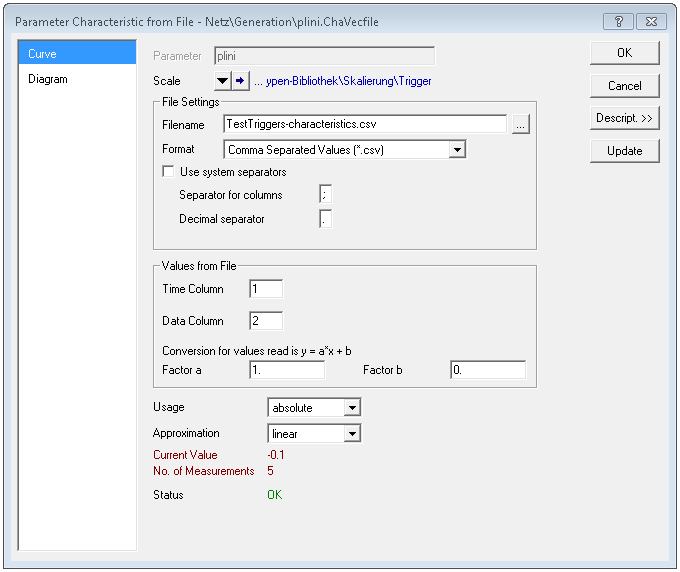
\includegraphics[width=0.9\textwidth]{characteristics_from_file}}
\vspace*{-2mm}
\caption{\pf window for defining a parameter characteristic from file.}
\label{fig:characteristics_from_file}
\vspace*{1em}
\centering{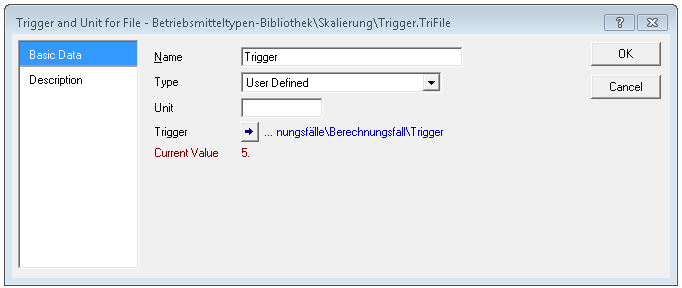
\includegraphics[width=0.85\textwidth]{trigger_for_file}}
\vspace*{-2mm}
\caption{\pf window for defining a trigger and unit for file.}
\label{fig:trigger_for_file}
\end{figure}

%\clearpage

To associate such a time series to a parameter do the following:
\begin{itemize}
  \item select the associated object (double-click)
  \item right-click the input field of the corresponding parameter to bring up the context menu
  \item first select \emph{Add Project Characteristic}, then \emph{Characteristic from File...}
  \item choose the previously created characteristic in the project browser
\end{itemize} 
Figure~\ref{fig:add_characteristics_from_file} shows how the context menus looks like for the example of associating a characteristic from file to the active power parameter of a general load.

\begin{figure}[h!]
\vspace*{2em}
\centering{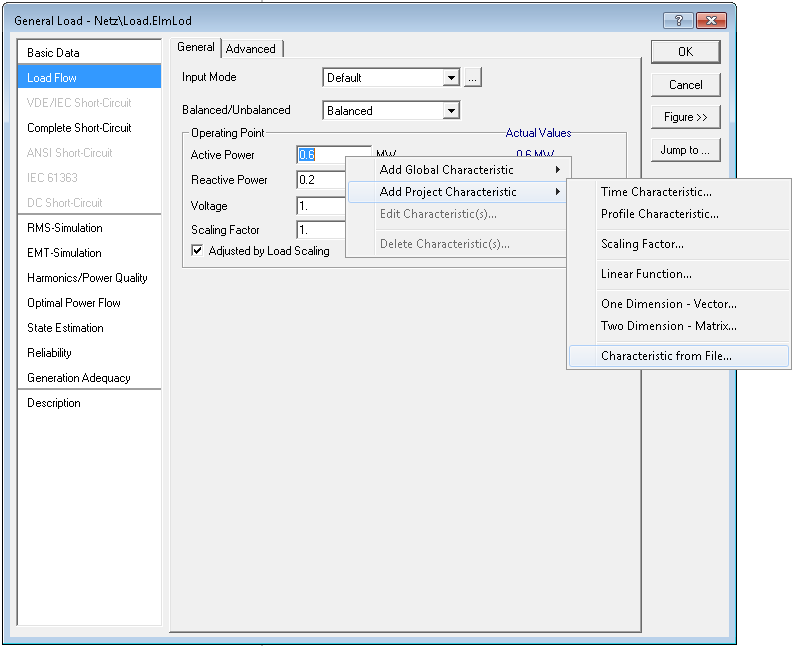
\includegraphics[width=0.9\textwidth]{add_characteristics_from_file}}
\caption{Context menus for associating a time series to a parameter.}
\label{fig:add_characteristics_from_file}
\end{figure}

\clearpage

\subsection{Exporting models using external time series and triggers}

In order to create an FMU from a PFD file that defines characteristics from files and triggers, a \python script has to be executed from the command prompt window (please refer to the \href{https://docs.python.org/2/faq/windows.html}{\python~FAQ} in case you need assistance with this).
Open the command prompt window and execute the script \texttt{powerfactory\_fmu\_create.py}:

\begin{verbatim}
python.exe <path_to_pf_fmu_dir>powerfactory_fmu_create.py [-h] [-v] 
  -m model_id -p pfd_file [-d pf_install_dir] [-i input_var_file]
  [-o output_var_file] [-t name:scale] [additional_file_1 ... ]
  [var1=start_val1 ...]
\end{verbatim}

The path to the \fmipp \pf FMU export utility directory \verb!<path_to_pf_fmu_dir>! may be relative or absolute.
Optional arguments are enclosed by squared brackets \verb![!$\,$\ldots\verb!]!, terms in angle brackets \verb!<!$\,$\ldots\verb!>! represent file paths.
  
\textit{Mandatory input arguments}:
  \begin{itemize}
    \item \verb!-m, --model-id!: specify FMU model identifier
    \item \verb!-p, --pfd-file!: path to PowerFactory PFD file
  \end{itemize}
  \textit{Optional input arguments}:
  \begin{itemize}
    \item \verb!-h, --help!: display the help screen
    \item \verb!-v, --verbose!: turn on log messages
    \item \verb!-l, --litter!: do not clean-up intermediate files
    \item \verb!-i, --input-var-file!: specify file containing list of input variable names
    \item \verb!-o, --output-var-file!: specify file containing list of output variable names
    \item \verb!-t, --trigger!: specify a trigger for advancing simulation time
    \item \verb!-d, --pf-install-dir!: path to \pf installation directory\footnote{It is usually not necessary to provide the path to the \pf installation directory, unless the FMU is intended to run on a another machine with a different installation directory path.}
  \end{itemize}
\end{enumerate}
Files containing lists of input and output variable names are expected to be in clear text, listing exactly one valid variable name per line.
As explained in Section~\ref{sec:export:naming_convention}, variable names are supposed to be of the  form \texttt{<object-type>.<object-name>.<parameter-name>}.

Triggers for simulation time advance need to be defined in the form \texttt{<name>:<scale>}.
The \texttt{name} has to be given according to the trigger's object name in the PFD file.
Times given to the FMU are interpreted as seconds, therefore the \texttt{scale} can be adjusted to match the trigger's internal unit of time (e.g., 60 for minutes or 3600 for hours).
Multiple triggers may be defined.

Additional files may be specified (e.g., CSV load profiles) that will be automatically copied to the FMU. The specified files paths may be absolute or relative.

Furthermore, start values for variables may be defined. For instance, to set a variable with the name \texttt{ElmLod.TestLoad.plini} to a value of 12.34, specify \texttt{ElmLod.TestLoad.plini=12.34} in the command line as optional argument.

Section~\ref{sec:examples:triggers} gives a concrete example of how to export such a model using time series and triggers as an FMU.


\section{Models using a \dplscript to define the time}

\subsection{Creating models using a \dplscript to define the time}
\label{sec:export:create_model_dplscript}

Parameters in \pf can be associated with 1-dimensional vectors, called \emph{Characteristic -- Vector} (\pf object of type \texttt{ChaVec}).
The actual value of the parameter can be changed by associating the elements of such a vector to a \emph{Time Scale} (\pf object of type \texttt{TriTime}) that maps each element to a specific point in time.
Time itself within the model can then be set with the help of a dedicated \dplscript.
Figure~\ref{fig:characteristics_from_vector} shows the setup window for such a vector characteristic, which defines the mapping of the values to the points in time defined by the time scale (defined via the \texttt{Scale} field).
Figure~\ref{fig:trigger_for_vector} shows the setup for the time scale itself.


\begin{figure}[h!]
\vspace*{1em}
\centering{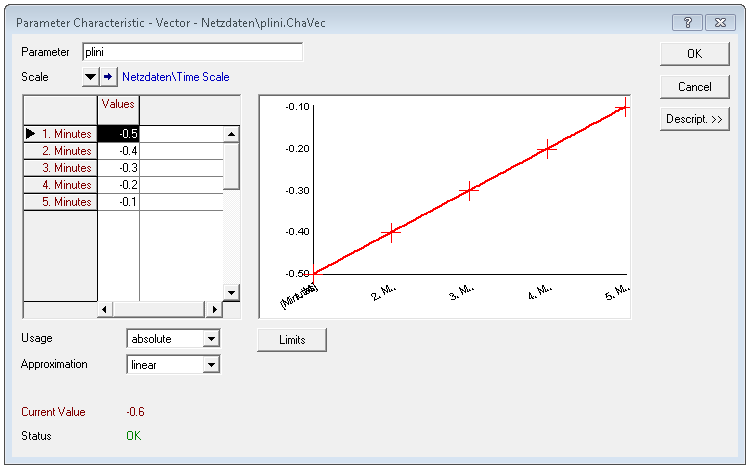
\includegraphics[width=0.9\textwidth]{characteristics_from_vector}}
\caption{\pf window for defining a parameter characteristic from a vector.}
\label{fig:characteristics_from_vector}
\vspace*{2em}
\centering{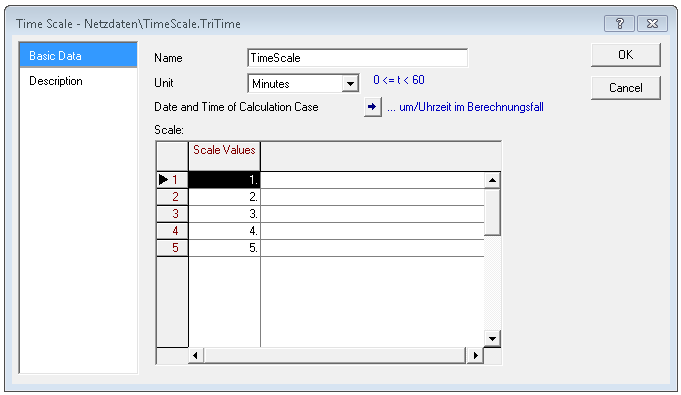
\includegraphics[width=0.85\textwidth]{trigger_for_vector}}
\caption{\pf window for defining a trigger and unit for a vector.}
\label{fig:trigger_for_vector}
\end{figure}

To associate such a vector characteristic to a parameter do the following:
\begin{itemize}
  \item select the associated object (double-click)
  \item right-click the input field of the corresponding parameter to bring up the context menu
  \item first select \emph{Add Project Characteristic}, then \emph{One Dimension -- Vector...}
  \item choose the previously created vector characteristic in the project browser
\end{itemize} 
Figure~\ref{fig:add_characteristic_vector} shows how the context menus looks like for the example of associating a characteristic from file to the active power parameter of a general load.

\begin{figure}[h!]
\vspace*{2em}
\centering{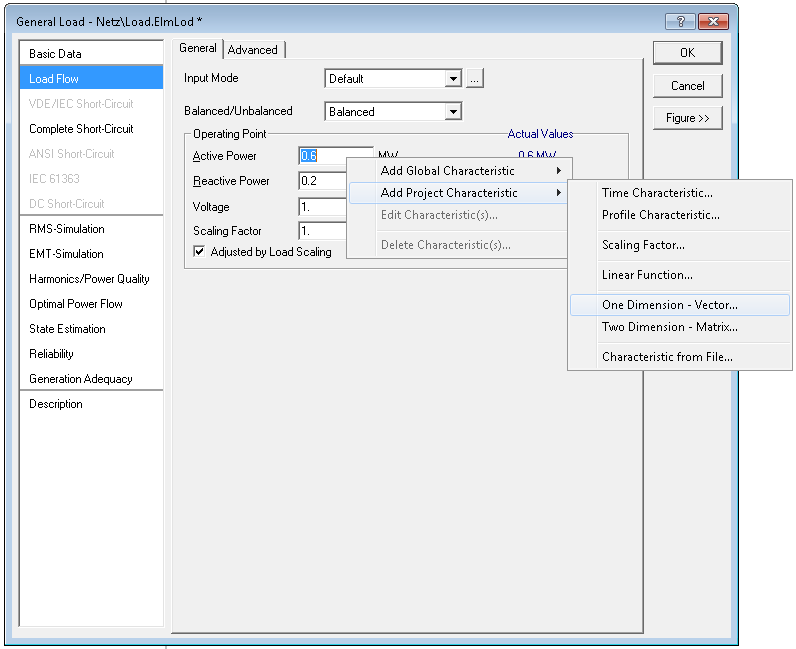
\includegraphics[width=0.9\textwidth]{add_characteristic_vector}}
\caption{Context menus for associating a vector characteristic to a parameter.}
\label{fig:add_characteristic_vector}
\end{figure}

\clearpage

In addition, the \dplscript for setting the time has to be provided.
Such a script could be of the following form:

\begin{Verbatim}[frame=single,commandchars=\\\{\}]

  \codeHighlightGreen{! Change date/time of active study case,}
  \codeHighlightGreen{! using the second of the year as input.}
  \codeHighlightGreen{!}
  \codeHighlightGreen{! ATTENTION: The script doesn't properly}
  \codeHighlightGreen{! handle simulation runs longer than one}
  \codeHighlightGreen{! year.}

  \codeHighlightBlue{object} \textcolor{black}{set_time;}

  \textcolor{black}{set_time =} \codeHighlightBlue{GetCaseObject}\textcolor{black}{(} \codeHighlightRed{'SetTime'} \textcolor{black}{);}

  \codeHighlightBlue{if} \textcolor{black}{( set_time ) \{}
  \textcolor{black}{  set_time:min = 0.0;}
  \textcolor{black}{  set_time:sec = 0.0;}
  \textcolor{black}{  set_time.SetTime( second_of_year * }\codeHighlightDarkRed{0.000277778}\textcolor{black}{ );}
  \textcolor{black}{\}}

\end{Verbatim}
The script's input is the second of the year, represented by variable \texttt{second\_of\_year} (compare to \dplscript setup in Figure~\ref{fig:dpl_script_setup})
The script calculates the hour of the year (by multiplication of $0.000277778 = 1 / 3600$) and and uses this value to set the model's time with the help of function \texttt{SetTime}.
\begin{figure}[h!]
\vspace*{1ex}
\centering{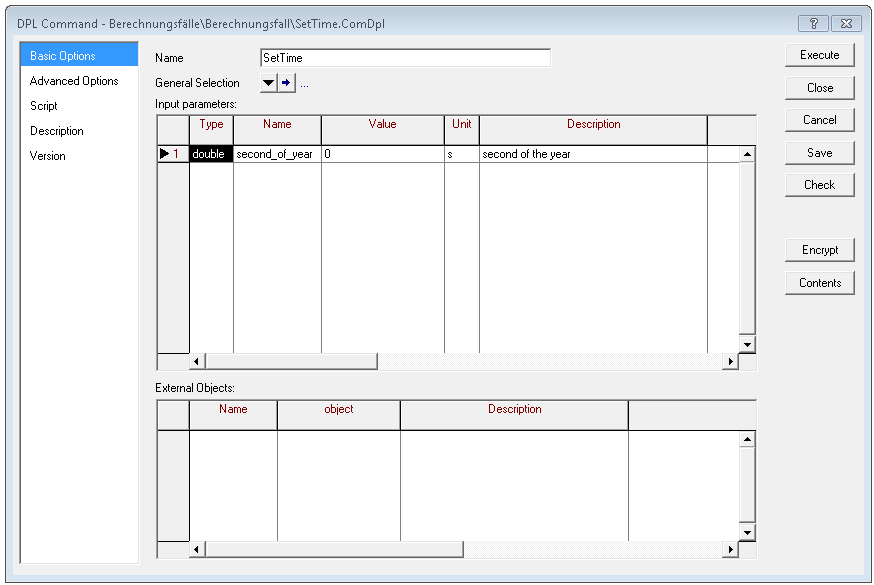
\includegraphics[width=0.95\textwidth]{dpl_script_setup}}
\vspace{-2mm}
\caption{\pf window for \dplscript setup.}
\label{fig:dpl_script_setup}
\end{figure}

\subsection{Exporting models using a \dplscript to define the time}

In order to create an FMU from a PFD file that uses a \dplscript to advance time, a \python script has to be executed from the command prompt window (please refer to the \href{https://docs.python.org/2/faq/windows.html}{\python~FAQ} in case you need assistance with this).
Open the command prompt window and execute the script \texttt{powerfactory\_fmu\_create.py}:

\begin{verbatim}
python.exe <path_to_pf_fmu_dir>powerfactory_fmu_create.py [-h] [-v] 
  -m model_id -p pfd_file [-d pf_install_dir] [-i input_var_file]
  [-o output_var_file] [-s name:scale:offset] [additional_file_1 ... ]
  [var1=start_val1 ...]
\end{verbatim}

The path to the \fmipp \pf FMU export utility directory \verb!<path_to_pf_fmu_dir>! may be relative or absolute.
Optional arguments are enclosed by squared brackets \verb![!$\,$\ldots\verb!]!, terms in angle brackets \verb!<!$\,$\ldots\verb!>! represent file paths.
  
\textit{Mandatory input arguments}:
  \begin{itemize}
    \item \verb!-m, --model-id!: specify FMU model identifier
    \item \verb!-p, --pfd-file!: path to PowerFactory PFD file
  \end{itemize}
  \textit{Optional input arguments}:
  \begin{itemize}
    \item \verb!-h, --help!: display the help screen
    \item \verb!-v, --verbose!: turn on log messages
    \item \verb!-l, --litter!: do not clean-up intermediate files
    \item \verb!-i, --input-var-file!: specify file containing list of input variable names
    \item \verb!-o, --output-var-file!: specify file containing list of output variable names
    \item \verb!-s, --dpl-script!: specify a \dplscript for advancing simulation time
    \item \verb!-d, --pf-install-dir!: path to \pf installation directory\footnote{It is usually not necessary to provide the path to the \pf installation directory, unless the FMU is intended to run on a another machine with a different installation directory path.}
  \end{itemize}
\end{enumerate}
Files containing lists of input and output variable names are expected to be in clear text, listing exactly one valid variable name per line.
As explained in Section~\ref{sec:export:naming_convention}, variable names are supposed to be of the form \texttt{<object-type>.<object-name>.<parameter-name>}.

A single \dplscript may be specified to advance simulation time in the form \texttt{<name>:<scale>:<offset>}.
The \texttt{name} has to be given according to the script's name in the PFD file.
Times given to the FMU are interpreted as seconds, therefore the \texttt{scale} and \texttt{offset} can be adjusted to match the \dplscript's internal representation of time (e.g., 60 for minutes or 3600 for hours).

Additional files may be specified that will be automatically copied to the FMU. The specified files paths may be absolute or relative.

Furthermore, start values for variables may be defined. For instance, to set a variable with the name \texttt{ElmLod.TestLoad.plini} to a value of 12.34, specify \texttt{ElmLod.TestLoad.plini=12.34} in the command line as optional argument.

Section~\ref{sec:examples:dplscript} gives a concrete example of how to export such a model using a \dplscript as an FMU.


\section{Writing additional output}
\label{sec:export:additional_output}

When using a \pf model within a co-simulation, it is possible to write additional simulation results from \pf that are not specified as FMU outputs.
To do so, simply add text files with file extension \texttt{.info} as additional files, containing a list of variable names in clear text, listing exactly one valid variable name per line (just like the input input/output variable name lists for creating an FMU).
For each of these files, a CSV file with the same name (but file extension \texttt{.csv}) will be generated during a simulation run, containing the simulated values of the variables defined in the \texttt{.info} file.
For instance, adding an additional file called \texttt{extra\_data.info} will at simulation time result in the creation of a file called \texttt{extra\_data.csv}.

\subsubsection*{Note:}
These \texttt{.info} files have to be specifically specified as additional files when creating an FMU!
% Copyright (c) 2015-2017, AIT Austrian Institute of Technology GmbH.
% REM All rights reserved. See file POWERFACTORY_FMU_LICENSE.txt for details.

\chapter{Examples}
\label{sec:examples}

This chapter gives examples of exporting FMUs from \pf models as described in Section~\ref{sec:export}.
All the examples use the same simple network model shown in Figure~\ref{fig:test_model}), but using different methods for defining time (trigger, \dplscript, RMS simulation).

These models are also included in the \emph{examples} folder of the \fmipp \pf Export Utility and can be used to create FMUs.
Section~\ref{sec:examples:results} provides expected simulation results as reference for testing these FMUs.

\begin{figure}[h!]
\vspace*{1em}
\centering{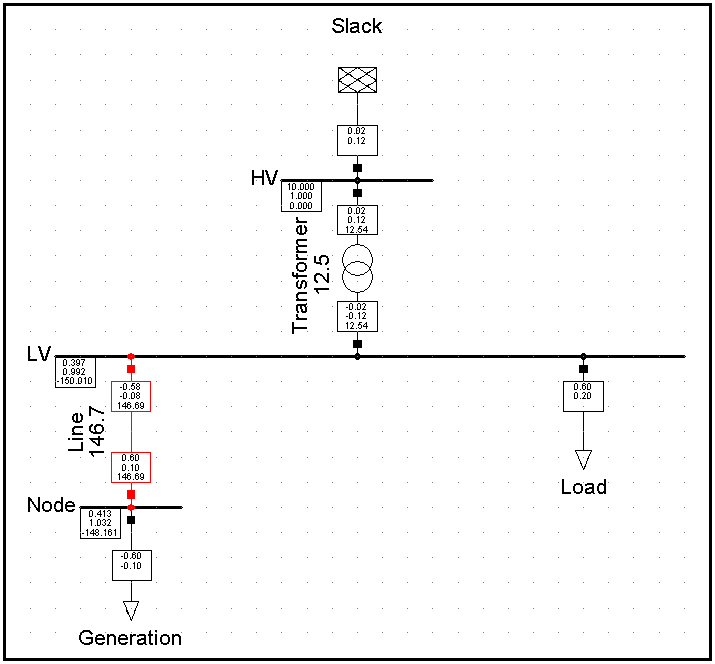
\includegraphics[width=0.74\textwidth]{test_model}}
\caption{Common power network model for example model.}
\label{fig:test_model}
\end{figure}


\section{Exporting a model using external time series and triggers}
\label{sec:examples:triggers}

An example for exporting a model using external time series and triggers can be found in subfolder \texttt{examples\symbol{92}triggers} of the installation directory.
It contains the following files:
\begin{itemize}
  \item \texttt{TestTriggers.pfd}: the \pf network model
  \item \texttt{TestTriggers-inputs.txt}: text file containing the lists of input variable names
  \item \texttt{TestTriggers-outputs.txt}: text file containing the lists of output variable names
  \item \texttt{TestTriggers-characteristics.csv}: text file containing a time series
\end{itemize}

\subsubsection*{The external time series}

In the power network model, the time series is associated with the active power (parameter \emph{plini}) of the general load named \emph{Generation}. The time series is provided in a simple text file, using semi-colons as column separators (compare to definition of \emph{File Settings} in Figure~\ref{fig:characteristics_from_file}):
\begin{Verbatim}[frame=single,commandchars=\\\{\}]
  \textcolor{black}{1;-0.5}
  \textcolor{black}{2;-0.4}
  \textcolor{black}{3;-0.3}
  \textcolor{black}{4;-0.2}
  \textcolor{black}{5;-0.1}
\end{Verbatim}

\subsubsection*{Exporting the FMU}

\begin{figure}[h!]
\vspace*{1em}
\centering{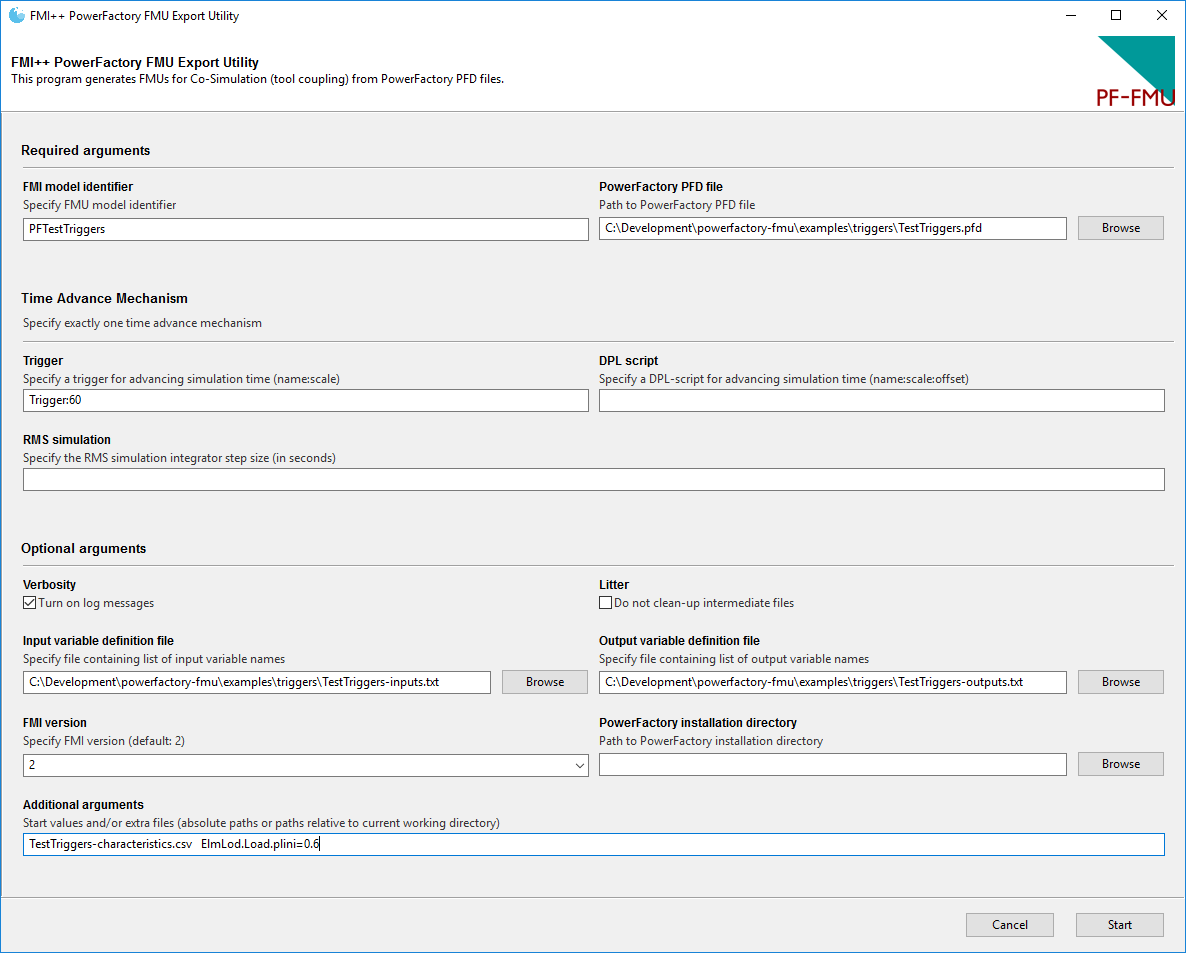
\includegraphics[width=\textwidth]{gui_create_trigger}}
\caption{Input to the graphical user interface for exporting a model using external time series and triggers.}
\label{fig:gui_create_trigger}
\end{figure}

To export the network model as FMU, specify the values in the graphical user interface as shown in Figure~\ref{fig:gui_create_trigger}.
When ready, click the \texttt{Start} button to create the FMU.
Alternatively, issue the following command in the command prompt window (directly from the directory containing the files):
\begin{verbatim}
python.exe ..\..\powerfactory_fmu_create.py -m PFTestTriggers \
  -i TestTriggers-inputs.txt -o TestTriggers-outputs.txt \
  -p TestTriggers.pfd -t Trigger:60 TestTriggers-characteristics.csv \
  ElmLod.Load.plini=0.6
\end{verbatim}
Some comments:
\begin{itemize}
  \item This command defines \emph{PFTestTriggers} as FMI model identifier.
  Hence, the resulting FMU is called \texttt{PFTestTriggers.fmu}.
  \item The command specifies one trigger called \texttt{Trigger}, with a scale of 60.
  This means that at master simulation time $T$ (in seconds), the associated characteristic in \pf will produce the time series value associated to $T/60$.
  For instance, at simulation time $T=180\,$s, the characteristic will produce the value $-0.3$ (compare with definition of time series above).
  \item The file containing the time series is explicitly declared as additional input file.
  In the \pf model, this file should be referred to directly by name, without a leading path (compare to Figure~\ref{fig:characteristics_from_file}).
  \item The active power (parameter name \emph{plini}) of the general load called \emph{Load} is initialized with the value $0.6$.
\end{itemize}

\newpage

\section{Exporting a model using a \dplscript}
\label{sec:examples:dplscript}

An example for exporting a model using a \dplscript can be found in subfolder  \texttt{examples\symbol{92}dplscript} of the installation directory.
It contains the following files:
\begin{itemize}
  \item \texttt{TestDPLScript.pfd}: the \pf network model
  \item \texttt{TestDPLScript-inputs.txt}: text file containing the lists of input variable names
  \item \texttt{TestDPLScript-outputs.txt}: text file containing the lists of output variable names
\end{itemize}

\subsubsection*{Associating a characteristic with the \dplscript}

In the power network model, a 1-dimensional characteristic is associated with the active power (parameter \emph{plini}) of the general load named \emph{Generation}.
Also, the \pf model contains a \dplscript that takes the second of the year as input to set the simulation time (compare with the \dplscript shown in Section~\ref{sec:export:create_model_dplscript}).

\subsubsection*{Exporting the FMU}

\begin{figure}[h!]
\vspace*{1em}
\centering{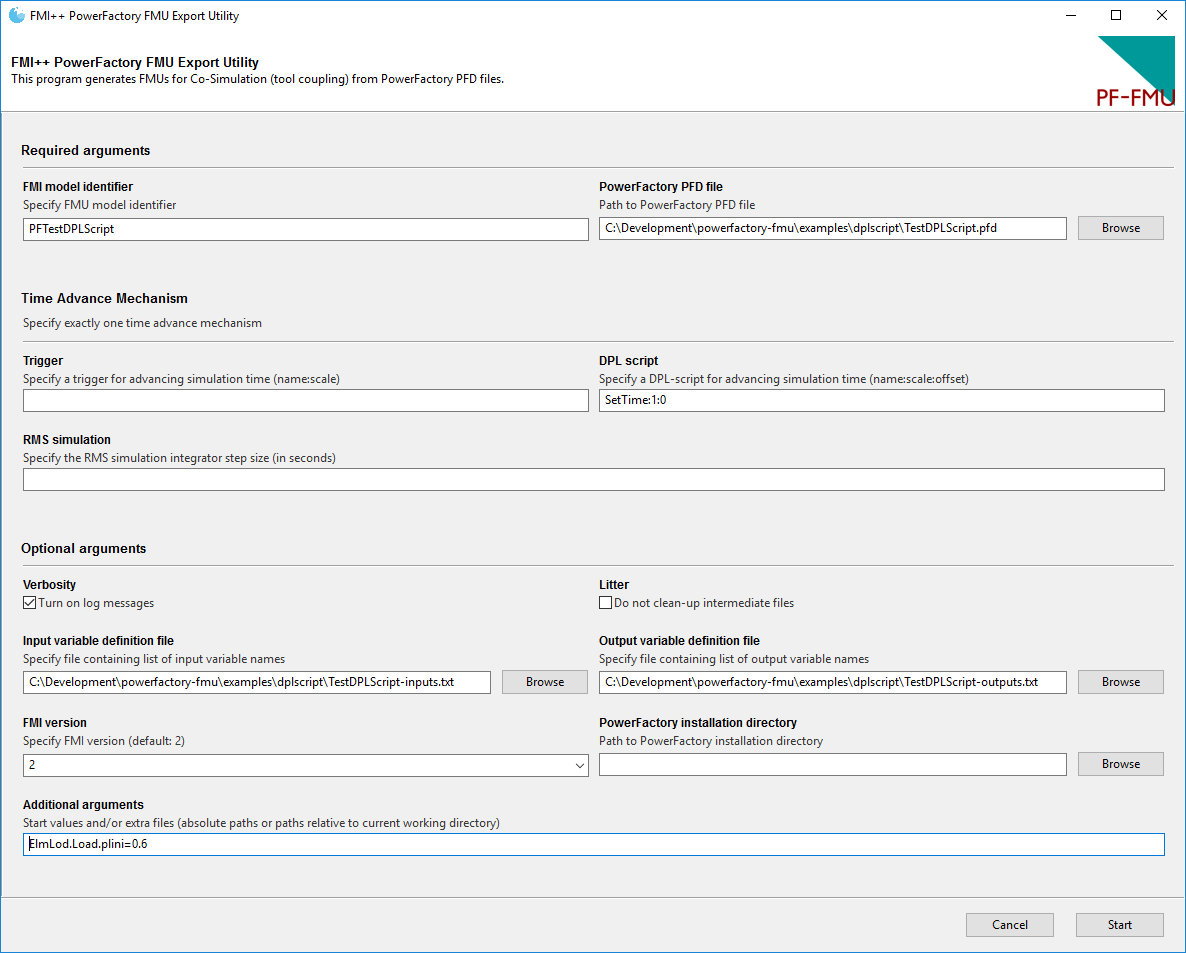
\includegraphics[width=\textwidth]{gui_create_dpl_script}}
\caption{Input to the graphical user interface for exporting a model using a \dplscript.}
\label{fig:gui_create_dpl_script}
\end{figure}

To export the network model as FMU, specify the values in the graphical user interface as shown in Figure~\ref{fig:gui_create_dpl_script}.
When ready, click the \texttt{Start} button to create the FMU.
Alternatively, issue the following command in the command prompt window (directly from the directory  containing the files):
\begin{verbatim}
python.exe ..\..\powerfactory_fmu_create.py -m PFTestDPLScript \
  -i TestDPLScript-inputs.txt -o TestDPLScript-outputs.txt \
  -p TestDPLScript.pfd -s SetTime:1:0 ElmLod.Load.plini=0.6
\end{verbatim}
Some comments:
\begin{itemize}
  \item This command defines \texttt{PFTestDPLScript} as FMI model identifier.
  Hence, the resulting FMU is called \texttt{PFTestDPLScript.fmu}.
  \item The command specifies the name of the \dplscript as \emph{SetTime}, with a scale of 1 and an offset of 0.
  This means that at master simulation time $T$ (in seconds), the associated \dplscript will be called with an input argument value of $T/1 + 0$.
  Since in this case the \dplscript expects the second of the year as input argument, simulation time 0 coincides with the beginning of the year.
  \item The active power (parameter name \emph{plini}) of the general load called \emph{Load} is initialized with the value $0.6$.
\end{itemize}


\newpage


\section{Exporting a model for RMS simulation}
\label{sec:examples:rmssim}

An example for exporting a model for RMS simulation can be found in subfolder \texttt{examples\symbol{92}rms} of the installation directory.
It contains the following files:
\begin{itemize}
  \item \texttt{TestRMS.pfd}: the \pf model
  \item \texttt{TestRMS-inputs.txt}: text file containing the lists of input variable names
  \item \texttt{TestRMS-outputs.txt}: text file containing the lists of output variable names
\end{itemize}

\subsubsection*{Model Structure}

The \pf model contains in subfolder \emph{Library} $\to$ \emph{User Defined Models} the following objects (see Figure~\ref{fig:example_rms_model_browser}):
\begin{itemize}
  \item \emph{ControllerForTwoLoads}: This \dslmodel (type \texttt{BlkDef}) defines two output signals, \emph{outPext1} and \emph{outPext2}, and two parameters, \emph{Pext1} and \emph{outPext2}, see Figure~\ref{fig:controller_for_two_loads}.
  In this simple example, the output signals are a direct "feedthrough" of the values of the parameters, as defined by the model's DSL equation (see Figure~\ref{fig:controller_for_two_loads_equ}).
  \item \emph{FMIAdapter}: block-definition of compiled \dslmodel FMIAdapter (see Section~\ref{sec:export:create_model_rms})
  \item \emph{FMIAdapterConfig}: composite model frame (type \texttt{BlkDef}) defining slots for the FMIAdapter, the controller and two loads as well as the connections between the controller and the loads, see Figure\ref{fig:fmiadapterconfig_composite_frame_2}
\end{itemize}

Furthermore, Figure~\ref{fig:example_rms_model_browser} shows that subfolder \emph{Network Model} $\to$ \emph{Network Data} $\to$ \emph{Grid} contains a composite model called \emph{FMIAdapterImplementation} (type \texttt{ElmComp}, see Figure~\ref{fig:fmiadapterconfig_composite_model}), which implements the composite frame FMIAdapterConfig.
It also contains common models (type \texttt{ElmDsl}) that implement the {\dslmodel}s defining the FMIAdapter and the ControllerForTwoLoads.
See for example Figure~\ref{fig:controllerinstance}, which shows the definition of common model \emph{ControllerInstance}.

\begin{figure}[h!]
%\vspace*{2em}
\centering{\fbox{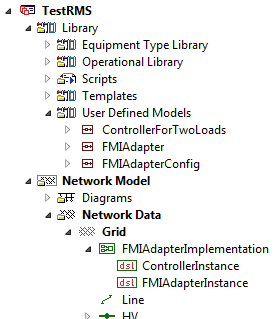
\includegraphics[width=0.45\textwidth]{example_rms_model_browser}}}
\caption{View of the data manager for \pf model TestRMS.}
\label{fig:example_rms_model_browser}
\end{figure}

\begin{figure}[h!]
\vspace*{1em}
\centering{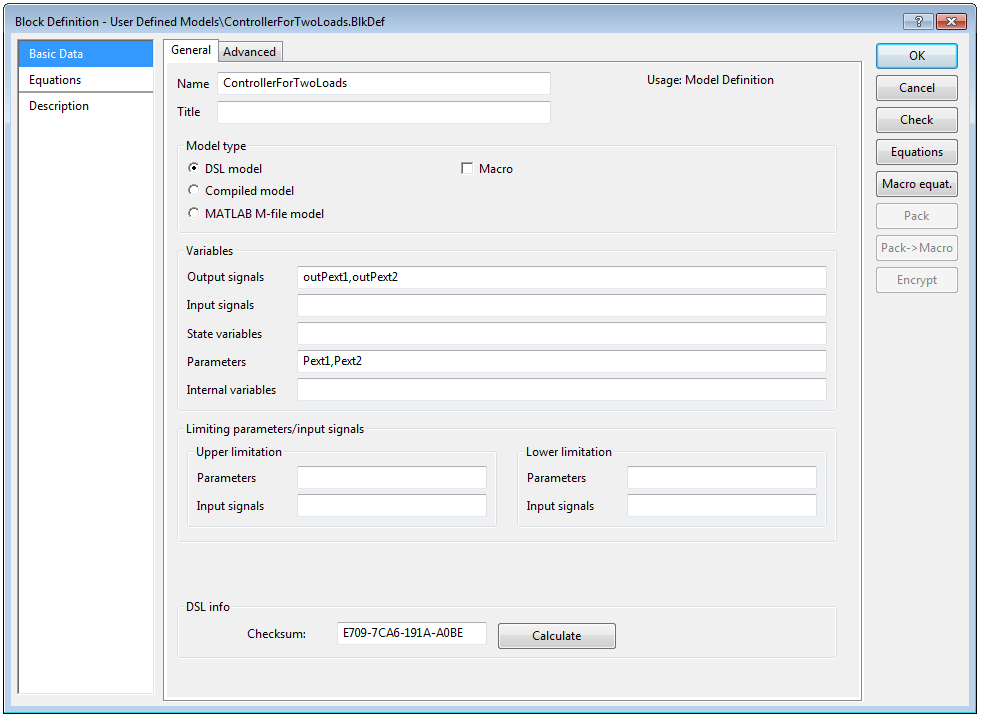
\includegraphics[width=0.98\textwidth]{controller_for_two_loads}}
\caption{Model definition of controller, including definition of output signals and parameters.}
\label{fig:controller_for_two_loads}
\end{figure}

\begin{figure}[h!]
\vspace*{2em}
\begin{Verbatim}[frame=single,commandchars=\\\{\}]
  \codeHighlightGreen{! Initial conditions for output signals.}
  \codeHighlightBlue{inc}\textcolor{black}{(outPext1) = Pext1}
  \codeHighlightBlue{inc}\textcolor{black}{(outPext2) = Pext2}

  \codeHighlightGreen{! Associate output signals with model parameters.}
  \textcolor{black}{outPext1 = Pext1}
  \textcolor{black}{outPext2 = Pext2}
\end{Verbatim}
\vspace*{-2ex}
\caption{DSL equations of controller.}
\label{fig:controller_for_two_loads_equ}
\end{figure}


\begin{figure}[h!]
\vspace*{1em}
\centering{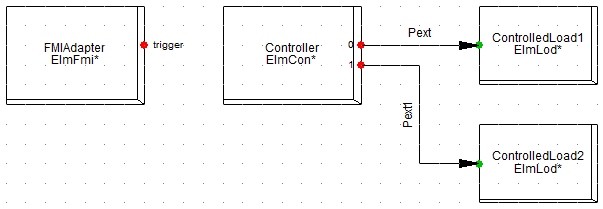
\includegraphics[width=0.7\textwidth]{fmiadapterconfig_composite_frame}}
\caption{Composite frame including \dslmodel FMIAdapter and a controller connected to two loads.}
\label{fig:fmiadapterconfig_composite_frame_2}
\end{figure}

\clearpage

\subsubsection*{Sending simulation events}

File \texttt{TestRMS-inputs.txt} contains the definition of two input variables:
\begin{Verbatim}[frame=single,commandchars=\\\{\}]
  \textcolor{black}{EvtParam.Controller.Pext1}
  \textcolor{black}{EvtParam.Controller.Pext2}
\end{Verbatim}
According to the naming convention (see Section~\ref{sec:naming_convention:sim_evt}), these two input variables correspond to simulation events.

When a new value is set for one of these two input variables at a synchronization point during the simulation, a simulation event is immediately issued in \pf.
The instance of the FMIAdapter model (in this example common model FMIAdapterInstance) will send the event to the corresponding slot of the composite frame that it belongs to (in this example slot Controller of composite frame FMIAdapterConfig).
Then the parameters of the model associated to this slot will be set to the new value (in this example parameters Pext1 or Pext2 of \dslmodel ControllerForTwoLoads).
Depending on the settings of \pf (mainly the integrator step size), the event will be executed within a short delay as soon as the next simulation step is started.

\begin{figure}[h!]
\vspace*{2em}
\centering{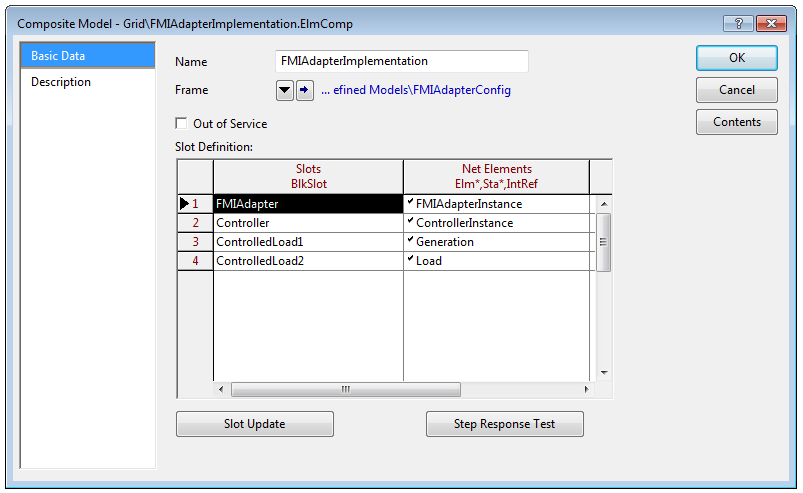
\includegraphics[width=0.98\textwidth]{fmiadapterconfig_composite_model}}
\caption{Definition of composite model FMIAdapterImplementation, implementing the composite frame (FMIAdapterConfig) and assigning the slots to common models and network elements.}
\label{fig:fmiadapterconfig_composite_model}
\end{figure}

\newpage

\begin{figure}[h!]
\vspace*{2em}
\centering{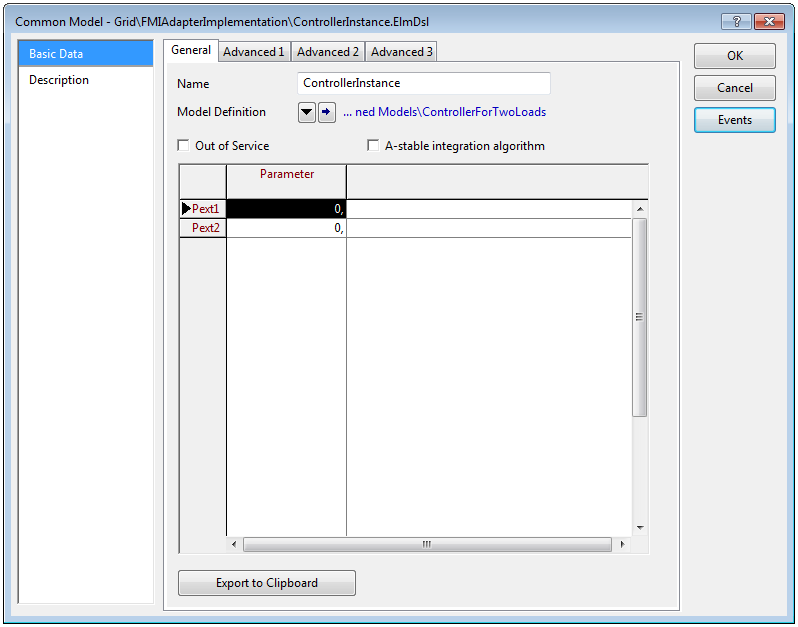
\includegraphics[width=0.98\textwidth]{controllerinstance}}
\caption{Definition of common model ControllerInstance, implementing \dslmodel ControllerForTwoLoads for common model FMIAdapterImplementation.}
\label{fig:controllerinstance}
\end{figure}

\subsubsection*{Exporting the FMU}

\begin{figure}[h!]
\vspace*{1em}
\centering{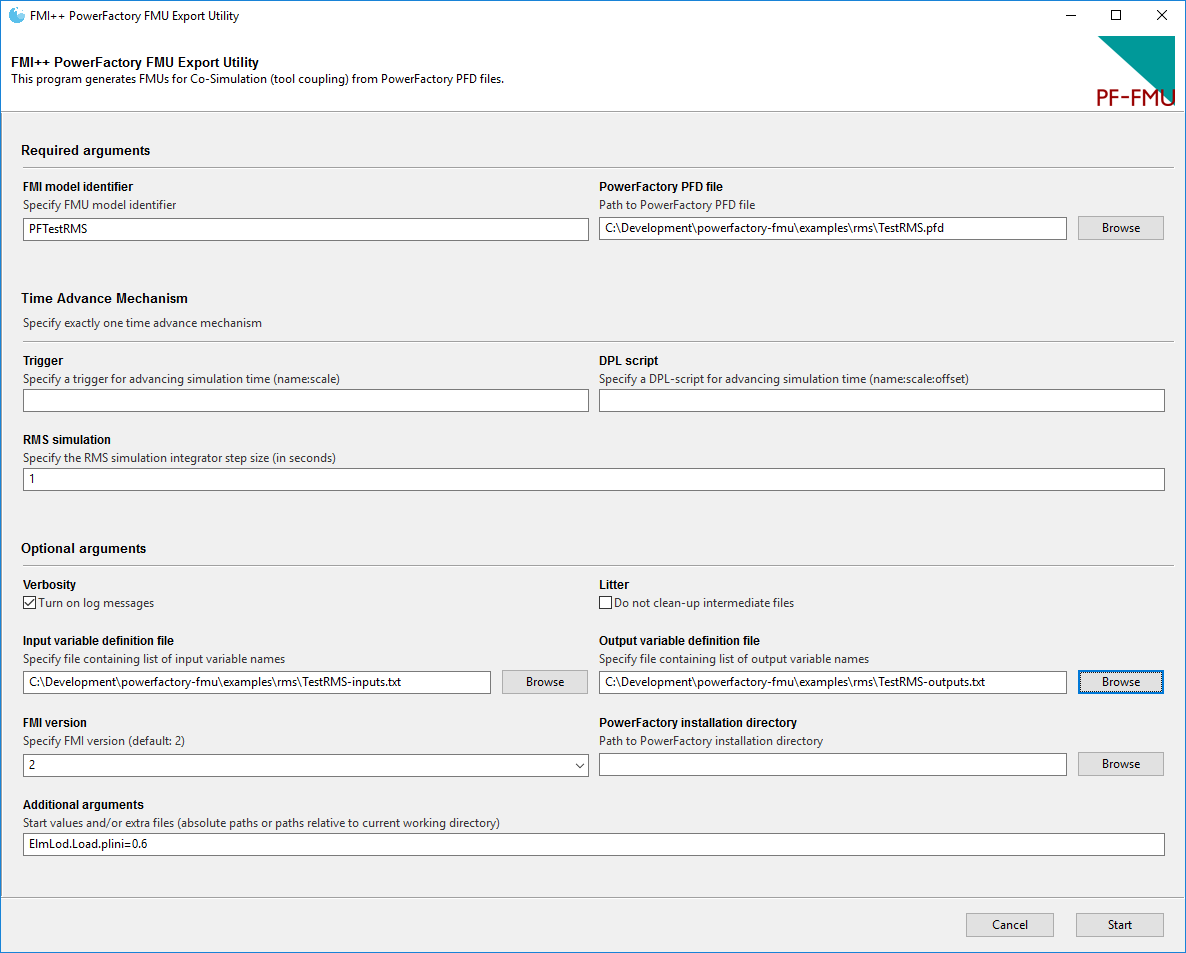
\includegraphics[width=\textwidth]{gui_create_rms}}
\caption{Input to the graphical user interface for exporting a model for RMS simulation}
\label{fig:gui_create_rms}
\end{figure}

To export the network model as FMU, specify the values in the graphical user interface as shown in Figure~\ref{fig:gui_create_rms}.
When ready, click the \texttt{Start} button to create the FMU.
Alternatively, issue the following command in the command prompt window (directly from the directory  containing the files):
\begin{verbatim}
python.exe ..\..\powerfactory_fmu_create.py -m PFTestRMS \
  -i TestRMS-inputs.txt -o TestRMS-outputs.txt \
  -p TestRMS.pfd -r 1 ElmLod.Load.plini=0.6
\end{verbatim}
Some comments:
\begin{itemize}
  \item This command defines \emph{PFTestRMS} as FMI model identifier.
  Hence, the resulting FMU is called \texttt{PFTestRMS.fmu}.
  \item The command specifies an integrator step size of 1~second for the RMS simulation.
  \item The active power (parameter name \emph{plini}) of the general load called \emph{Load} is initialized with the value $0.6$.
\end{itemize}


\newpage

\section{Reference results}
\label{sec:examples:results}

The examples above are included in the \emph{examples} folder of the \fmipp \pf Export Utility and can be used to create FMUs for testing.
This section provides expected simulation results as reference for testing the created FMUs.

\subsection{Results for using the model with an external time series and a trigger}
\label{sec:examples:results_trigger}

When properly exported and used within a co-simulation framework (without any further inputs), the results in Table~\ref{tab:examples:trigger_outputs} should be observed for output variable \texttt{ElmTerm.Node.m:u} (FMI value reference 1001):

\begin{table}[h!]
\centering{\begin{tabular}{|c|c|}
   \hline 
   simulation time & \texttt{ElmTerm.Node.m:u} \\ 
   \hline \hline 
   0~min & 1.03205 \\ \hline 
   1~min & 1.02631 \\ \hline 
   2~min & 1.02036 \\ \hline 
   3~min & 1.01422 \\ \hline 
   4~min & 1.00785 \\ \hline 
   5~min & 1.00125 \\ \hline
\end{tabular}}
\caption{Expected outputs from model with an external time series and a trigger.}
\label{tab:examples:trigger_outputs}
\end{table}



\subsection{Results for using the model with a \dplscript}
\label{sec:examples:results_dplscript}

When properly exported and used within a co-simulation framework (without any further inputs), the same results as for the model with an external time series and a trigger should be observed (see Section~\ref{sec:examples:results_trigger} above).


\subsection{Results for using the model for RMS simulation}
\label{sec:examples:results_rms}

When properly exported and used within a co-simulation framework, the inputs given in Table~\ref{tab:examples:rms_inputs} should be applied.
Table~\ref{tab:examples:rms_outputs} lists the results that should be observed.
Please note that the synchronization points for setting inputs are not the same as for reading outputs.


\begin{table}[h!]
\centering{\begin{tabular}{|c|c|c|}
    \hline 
    simulation time & \texttt{EvtParam.Controller.Pext1} & \texttt{EvtParam.Controller.Pext2} \\ 
    \hline \hline 
    0~s & -1.0 & 2.0 \\ \hline 
    60~s & -0.5 & 0.5 \\ \hline 
    120~s & -1.0 & 1.0 \\ \hline 
    180~s & -1.5 & 1.5 \\ \hline 
    240~s & -2.0 & 2.0 \\ \hline 
\end{tabular}}
\caption{Inputs for RMS simulation.}
\label{tab:examples:rms_inputs}

\vspace*{2ex}

\centering{\begin{tabular}{|c|c|c|}
    \hline 
    simulation time & \texttt{ElmTr2.Transformer.m:P:buslv} & \texttt{ElmLod.Generation.m:I1:bus1} \\ 
    \hline \hline 
    30~s & -0.89504 & 1.48945 \\ \hline 
    90~s & 0.01403 & 0.73285 \\ \hline 
    150~s & 0.05495 & 1.50371 \\ \hline 
    210~s & 0.11969 & 2.30737 \\ \hline 
    270~s & 0.20321 & 3.13618 \\ \hline
\end{tabular}}
\caption{Expected outputs from RMS simulation.}
\label{tab:examples:rms_outputs}
\end{table}


% Copyright (c) 2015-2017, AIT Austrian Institute of Technology GmbH.
% All rights reserved. See file POWERFACTORY_FMU_LICENSE.txt for details.

\chapter{Troubleshooting}

Sorry, nothing yet.
However, please feel free to \href{http://sourceforge.net/projects/powerfactory-fmu/support}{provide feedback to the developers}.
\chapter{Appendix}

\section{The \fmipp \pf Export Utility License}
\label{pf_fmu_license}

Copyright (c) 2015, AIT Austrian Institute of Technology GmbH. All
rights reserved.

Redistribution and use in source and binary forms, with or without
modification, are permitted provided that the following conditions are
met:

\begin{itemize}
\itemsep1pt\parskip0pt\parsep0pt
\item
  Redistributions of source code must retain the above copyright notice,
  this list of conditions and the following disclaimer.
\item
  Redistributions in binary form must reproduce the above copyright
  notice, this list of conditions and the following disclaimer in the
  documentation and/or other materials provided with the distribution.
\end{itemize}

THIS SOFTWARE IS PROVIDED BY THE COPYRIGHT HOLDERS AND CONTRIBUTORS ``AS
IS'' AND ANY EXPRESS OR IMPLIED WARRANTIES, INCLUDING, BUT NOT LIMITED
TO, THE IMPLIED WARRANTIES OF MERCHANTABILITY AND FITNESS FOR A
PARTICULAR PURPOSE ARE DISCLAIMED. IN NO EVENT SHALL THE COPYRIGHT
HOLDER OR CONTRIBUTORS BE LIABLE FOR ANY DIRECT, INDIRECT, INCIDENTAL,
SPECIAL, EXEMPLARY, OR CONSEQUENTIAL DAMAGES (INCLUDING, BUT NOT LIMITED
TO, PROCUREMENT OF SUBSTITUTE GOODS OR SERVICES; LOSS OF USE, DATA, OR
PROFITS; OR BUSINESS INTERRUPTION) HOWEVER CAUSED AND ON ANY THEORY OF
LIABILITY, WHETHER IN CONTRACT, STRICT LIABILITY, OR TORT (INCLUDING
NEGLIGENCE OR OTHERWISE) ARISING IN ANY WAY OUT OF THE USE OF THIS
SOFTWARE, EVEN IF ADVISED OF THE POSSIBILITY OF SUCH DAMAGE.


\section{The \fmipp License}
\label{fmipp_license}

Copyright (c) 2013, AIT Austrian Institute of Technology GmbH. All
rights reserved.

Redistribution and use in source and binary forms, with or without
modification, are permitted provided that the following conditions are
met:

\begin{itemize}
\itemsep1pt\parskip0pt\parsep0pt
\item
  Redistributions of source code must retain the above copyright notice,
  this list of conditions and the following disclaimer.
\item
  Redistributions in binary form must reproduce the above copyright
  notice, this list of conditions and the following disclaimer in the
  documentation and/or other materials provided with the distribution.
\end{itemize}

THIS SOFTWARE IS PROVIDED BY THE COPYRIGHT HOLDERS AND CONTRIBUTORS ``AS
IS'' AND ANY EXPRESS OR IMPLIED WARRANTIES, INCLUDING, BUT NOT LIMITED
TO, THE IMPLIED WARRANTIES OF MERCHANTABILITY AND FITNESS FOR A
PARTICULAR PURPOSE ARE DISCLAIMED. IN NO EVENT SHALL THE COPYRIGHT
HOLDER OR CONTRIBUTORS BE LIABLE FOR ANY DIRECT, INDIRECT, INCIDENTAL,
SPECIAL, EXEMPLARY, OR CONSEQUENTIAL DAMAGES (INCLUDING, BUT NOT LIMITED
TO, PROCUREMENT OF SUBSTITUTE GOODS OR SERVICES; LOSS OF USE, DATA, OR
PROFITS; OR BUSINESS INTERRUPTION) HOWEVER CAUSED AND ON ANY THEORY OF
LIABILITY, WHETHER IN CONTRACT, STRICT LIABILITY, OR TORT (INCLUDING
NEGLIGENCE OR OTHERWISE) ARISING IN ANY WAY OUT OF THE USE OF THIS
SOFTWARE, EVEN IF ADVISED OF THE POSSIBILITY OF SUCH DAMAGE.

\section{The \boost Software License}
\label{boost_license}

Version 1.0 - August 17th, 2003

Permission is hereby granted, free of charge, to any person or organization
obtaining a copy of the software and accompanying documentation covered by
this license (the "Software") to use, reproduce, display, distribute,
execute, and transmit the Software, and to prepare derivative works of the
Software, and to permit third-parties to whom the Software is furnished to
do so, all subject to the following:

The copyright notices in the Software and this entire statement, including
the above license grant, this restriction and the following disclaimer,
must be included in all copies of the Software, in whole or in part, and
all derivative works of the Software, unless such copies or derivative
works are solely in the form of machine-executable object code generated by
a source language processor.

THE SOFTWARE IS PROVIDED "AS IS", WITHOUT WARRANTY OF ANY KIND, EXPRESS OR
IMPLIED, INCLUDING BUT NOT LIMITED TO THE WARRANTIES OF MERCHANTABILITY,
FITNESS FOR A PARTICULAR PURPOSE, TITLE AND NON-INFRINGEMENT. IN NO EVENT
SHALL THE COPYRIGHT HOLDERS OR ANYONE DISTRIBUTING THE SOFTWARE BE LIABLE
FOR ANY DAMAGES OR OTHER LIABILITY, WHETHER IN CONTRACT, TORT OR OTHERWISE,
ARISING FROM, OUT OF OR IN CONNECTION WITH THE SOFTWARE OR THE USE OR OTHER
DEALINGS IN THE SOFTWARE.

\section{Version History}

\begin{itemize}
  \item v0.1: first release version
  \item v0.2: support installation paths containing spaces (e.g., \texttt{C:\symbol{92}Program Files\symbol{92}powerfactory-fmu}).
  \item v0.3: ducumented extra output feature, allow comments in input/output variable name lists, added a reminder in the installation script to add the \pf installation directory to the Windows path, avoid crashes in case the \pf installation directory has not been added to the Windows path
  \item v0.4: update to \pf 2016 (using Visual Studio Express 2013)
  \item v0.5: update to Python~3
\end{itemize}



%----------------------------------------------------------------------------------------
%	INDEX
%----------------------------------------------------------------------------------------

%\cleardoublepage
%\phantomsection
%\setlength{\columnsep}{0.75cm}
%\addcontentsline{toc}{chapter}{\textcolor{ocre}{Index}}
%\printindex

%----------------------------------------------------------------------------------------

\end{document}
